\section{Implementierung}\label{sec:implementierung}
%TOTO LEFTOVER: 
%QUIZ
%HTTPS
%WLAN
Das folgende Kapitel wird Einblicke in die Entwicklung der Software im Rahmen des Projekts geben. 
Dabei wird iterativ chronologisch die Vorgehensweise schriftlich reflektiert und an mehreren Stellen 
zum besseren Verständnis auch ein Einblicke in den Sourcecode gegeben. Anknüpfend werden etwaige Probleme bei der Implementierung aufgezeigt sowie mögliche Lösungen diskutiert. 

\subsection{Implementierung der Server-Software}\label{sec:implementserver}
Aufbauend auf das Entwurfs Kapitel soll die Server-Software mit \emph{Node.js} und \emph{Express} als Hauptkomponente entwickelt werden. Dazu wird zunächst im folgenden Abschnitt \ref{sec:implementexpress} der HTTP Server grundlegend konfiguriert und anschließend dessen Routen im darauffolgenden Abschnitt \ref{sec:anlegrouten} angelegt. 

\subsection{ExpressJS Setup}\label{sec:implementexpress}
Nachdem das Projekt grundlegend mit dem Befehl \texttt{npm init} initialisiert wurde,
kann ExpressJS einfach über den \emph{Node Packet Manager} (NPM) hinzugefügt werden. 
Zusätzlich wird das NPM Modul \emph{IP} genutzt um die aktuelle IP-Adresse des Host-Computers automatisch zu ermitteln und
den \emph{Express}-Server auf dieser lauschen zu lassen. Dies wird im folgendem Code-Listing getan:
\begin{lstlisting}[caption=Errichtung des Webservers]
const app = express();
const server = app.listen(3000, server_ip, function () {
logger.log({ level: 'info', message: `Hello! The Server is running on ${server_ip}!`});
});
\end{lstlisting}
Der Server lauscht auf der IP Adresse des Netzwerk-Adapters der Maschine auf dem er ausgeführt wird. Zusätzlich wurde der Port 3000 spezifiziert. Dies kann je nach Konfiguration auf den Standard HTTP Port 80 resp. 443 geändert werden, sollte Verschlüsselung eingerichtet sein (HTTPS).
\\
Anschließend können nun die Routen eingerichtet werden.

\subsection{Autarkes WLAN}\label{sec:eigeneswlan}
Um einen Stand-Alone Betrieb\footnote{Stand-Alone meint einen Betrieb unabhänging von ggf. vorhandenen Netzwerkinfrastruktur am Einsatzort} der Software zu ermöglichen, wird als Lösung der Betrieb eines eigens aufgebautem kabellosen Netzwerkes (WLAN/Wifi) angestrebt. Folgende mögliche Lösungsszenarien wurden ausgearbeitet.
\begin{enumerate}
	\item \textbf{Einfach}: Als einfachste Lösung hat sich der Betrieb eines lokalen WLANs über ein Smartphone oder Laptop herausgestellt. Nahezu jedes Smartphone bzw. jeder Laptop lässt das Generieren eines WLAN Zugangspunktes für andere Geräte zu. Alle Clients und der Server selbst werden mit diesem Netzwerk verbunden. Dies Verbindung wurde getestet und ein Betrieb war möglich. Da hierbei aber auch die Internetverbindung des Zugangspunktes freigegeben wird, was ggf. unerwünscht sein kann, würde es sich anbieten eine spezielle "`Companion App"' zu entwickeln und für \emph{Android} / \emph{iOS} basierte Smartphones zu anzubieten. Diese App könnte automatisch einen WLAN-Hotspot erstellen und den Netzwerkverkehr ins Internet eventuell limitieren. Gleiches gilt analog für windows- oder unixbasierte Computer, ist aber problematischer, siehe dazu nächster Listenpunkt.
	\item \textbf{Speziell}: Um auf einem Computer vollautomatisch einen WLAN Hotspot zu genieren, bedarf es Administrator Privilegien sowie genauere Kenntnisse über den verwendeten Netzwerkadapter. NodeJS selbst bietet nur eingeschränkt Möglichkeiten an, diese Aufgabe autark zu übernehmen, könnte aber ggf. eventuelle Shell-Skripte triggern. Unter \emph{Microsoft Windows 7} und höheren Versionen, gibt es mit den NPM Paket \texttt{node-hotspot} auch die Möglichkeit, dies direkt mit \emph{Node.js} zu erledigen. Dieses Paket wird in die zu entwickelnde Software integriert und soll anschließend unter einer \emph{Microsoft Windows} Umgebung das generieren eines WLAN Hotspots / Zugangspunktes ermöglichen. Zur Verwendung werden entsprechende Steuerungsoptionen in Einstellungsbereich im Lehrkraft Backend integriert. Die interne Steuerung erfolgt über Routen (siehe auch Abschnitt \ref{sec:anlegrouten}).
	
Wird die Applikation in einer vorhandenen Netzwerkinfrastruktur betrieben, ist ein Betrieb in jedem Falle gewährleistet. Ist diese Vorraumsetzung nicht gegeben, könnte ein mobiler WLAN-Router genutzt werden, sollte keine ausreichende Infrastruktur vorhanden sein. Dieser müsste einmalig konfiguriert werden und ist anschließend in der Lage die Serverapplikation für Clients ansprechbar zu machen. Ein solches Gerät gibt es bereits ab ca. 10 Euro zu erwerben.
\end{enumerate} 

\subsection{Verschlüsselung}\label{sec:encrypted}
Um eine verschlüsselte Kommunikation zwischen Server und Clients zu gewährleisten, sollte der Datenaustausch nicht über das HTTP Protokoll,  sondern über das HTTPS Protokoll erfolgen. Um HTTPS allerdings sinnvoll nutzen zu können, ist ein Zertifikat von einer Zertifizierungsstelle (CA) notwendig, was, mit Kosten verbunden ist. Das Zertifikat gewährleistet die Identität des Servers. Allerdings bietet der Anbieter \emph{Let's Encrypt} \cite{LetsEncrypt.org} kostenlose Zertifikate an, welche sich problemlos bei vorhandenem SSH-Zugang installieren lassen. Hier wird aber nur die Domain zertifiziert. Bezahlte Zertifikate von anderen CAs bieten im Vergleich höheren Support und es wird nicht nur die Domain an sich zertifiziert, sondern das ganzen Unternehmen an sich. Außerdem besteht ein Gewährleistungs- und Garantieanspruch gegenüber der CA \cite{Ali2019}. \\
Für den Intranet Betrieb können auch eigens ausgestellte Zertifikate genutzt werden, welche mit Shell-Programmen wie \texttt{openssl} generierbar sind \cite{Copes2018}. Allerdings warnen moderne Webbrowser den Nutzenden recht auffällig, dass die genutzte Verbindung dennoch nicht sicher ist, da dem Zertifikat nicht vertraut werden kann. Soll die Applikation rein im Intranet laufen, könnte die Schule alternativ eine Sub-Domain anlegen, welche nur aus dem Intranet erreichbar ist und ebenfalls durch ein signiertes Zertifikat geschützt ist. \\Der HTTPS Betrieb wurde erfolgreich getestet. Die Implementierung ist nicht aufwendig allerdings, birgt aber den o.g. Nachteil. Da das Intranet ein an sich abgeschlossenes Netzwerk ist, scheint der verschlüsselte Betrieb in diesem zunächst nicht wichtig, kann aber jederzeit realisiert werden und ist bei Betrieb im Internet als obligatorisch zu betrachten. 

\subsection{Anlegen der Routen}\label{sec:anlegrouten}

Grundlegend soll es folgende Routen auf dem Server geben:
\begin{itemize}
	\item \textbf{"`/"'}: Die Haupt Route, sie wird angesteuert, wenn der Server einfach unter seiner IP (oder eingerichteter Domain) kontaktiert wird. Hier wird anschließend die Rolle des Nutzers (Lehrender oder Schülerin/Schüler) abgefragt  und dementsprechend weitergeleitet.
	\item \textbf{"`/teacher"'}: Diese Route verweist auf den Lehrerbereich der Anwendung, man kann sie auch als Backendbereich bezeichnen. Alle hinter dieser Route liegende Routen bedürfen einer Authentifizierung seitens des Nutzenden.
	\item \textbf{"`/client"'}: Diese Route verweist grundlegend auf den Student Client. Aber auch der Presenter Client wird über diese Weiche aufgerufen. 
\end{itemize}
Neben diesen drei Hauptrouten existieren noch weitere Routen für das Error-Handling (z.B. "`404 - Seite nicht gefunden"') sowie besondere für die \emph{WebSocket}-Kommunikation, welche aber im Hintergrund genutzt werden.
Das Anlege der Routen ist mit folgendem Codeausschnitt durchgeführt:
\begin{lstlisting}[caption=Anlegen der Routen]
app.use('/teacher', teacherRoutes);
app.use('/client', clientRoutes);
app.use('/', mainRoutes);
\end{lstlisting}

\footnotesize{Die Route Module werden im Hauptmodul (app.js) referenziert und deren Zuständigkeit festgelegt.} \\ \\
\normalsize
Zu beachten ist: Die weiterführenden Routen werden in Dateien ausgelagert, um die Übersicht des Quelltextes zu wahren. Zudem sind auch diese Routen sog. Middleware-Funktionen. Dies wird im nächsten Abschnitt genauer beleuchtet. Daher ist auch die Reihenfolge wichtig, wie in Listing 2 dargestellt. Würde die \texttt{"`/"'}~Route als erstes angelegt werden, so würde diese alle folgenden, spezifischeren "`abfangen"'.  

\newpage
\subsection{Reflexion des MVC Schemas}\label{sec:mvc}
Da der Server grundlegend nach dem \emph{Model-View-Controller} Muster  arbeiten soll, gilt es dieses zu implementieren. Die folgende Tabelle \ref{tab:mvcschema} gibt einen Überblick über die anfallende Struktur:

\begin{table}[h!]
	\caption{MVC Struktur der Implementierung}
	\label{tab:mvcschema}
	\begin{tabular}{llll}
		
		\multicolumn{1}{c}{\textbf{Betrifft}}                         & \multicolumn{1}{c}{\textbf{Model}} & \multicolumn{1}{c}{\textbf{View(s)}}                                                                         & \multicolumn{1}{c}{\textbf{Controller}}                                            \\ \toprule
		Lehrende                                                        & user.js                             & \begin{tabular}[c]{@{}l@{}}teacher/new.pug\\ teacher/signup.pug\\ teacher/user-edit.pug\end{tabular}          & teacher.js                                                                          \\ \rowcolor[HTML]{EFEFEF} 
		\begin{tabular}[c]{@{}l@{}}Schülerinnen/\\ Schüler\end{tabular} & student.js                          & student.pug                                                                                                   & client.js                                                                           \\ 
		Lehreinheiten                                                   & eduSession.js                       & \begin{tabular}[c]{@{}l@{}}edusessions/*/*.pug\\ edusessions/index.pug\\ edusessions/running.pug\end{tabular} & \begin{tabular}[c]{@{}l@{}}session.js\\ quizzing.js\\ brainstorming.js\end{tabular} \\ \rowcolor[HTML]{EFEFEF} \midrule
	\end{tabular}
\footnotesize {
	\underline{Hinweis:} Zum Zwecke der Übersicht wurden einige interne Controller-Dateien nicht gelistet, wie z.B. der Error-Controller, welcher zwar eine View besitzt, jedoch kein Model. 
}
\end{table}

Nun sollen die entsprechenden Controller-Funktionen an die Routen gebunden werden. Entsprechende Unterrouten werden zu den aus Abschnitt \ref{sec:anlegrouten} bereits angelegten hinzugefügt. Im Sinne der Übersicht wird hierzu ein Routen-Ordner angelegt, welcher Routen-Module enthalten soll. 
Folgende Routen-Module werden angelegt: \\ \\
\textbf{routes/main.js}: Generelle Routen (Startseite etc.). \\
\textbf{routes/client.js}: Student Client / Presenter Client relevanten Routen.\\
\textbf{routes/teacher.js}: Alle für das Backend resp. Lehrerbereich relevanten Routen.\\ \\
Es folgt ein Codebeispiel (Listing 3) aus der Datei \texttt{routes/client.js}. 
\begin{lstlisting}[caption=Unterrouten und Controlleranbindung]
// 3rd Party Imports
const express = require('express');
const router = express.Router();
// App Imports
const clientController = require('../controllers/client');
const isAuth = require('../middleware/is-auth');
// Presenter & Student Clients
router.get('/presenter/:sessionId', isAuth, clientController.getPresenter);
router.get('/student', clientController.getStudent);
router.get('/', clientController.getStudent);
module.exports = router;
\end{lstlisting}
\newpage
Zur Verdeutlichung wird anknüpfend die in Zeile 10 des vorangegangen Listings 3, die Funktion \texttt{getStudent} des Controllers in Listing 4 gezeigt:
\begin{lstlisting}[caption=GET Funktion des Student Controllers]
// GET => /client/student
exports.getStudent = (req, res, next) => {

return res.render('client/student',
	{
		docTitle: 'Student | Node ICT',
		ipAdd: ip.address(),
	});
};
\end{lstlisting}
 
 \subsection{Einrichtung der Datenbank}
 Die SQL Datenbank \emph{SQLite}  und der Object-Relationship-Mapper \emph{Sequelize} können unkompliziert über NPM dem Projekt hinzugefügt werden.  
 Nach diesem Schritt kann die Anbindung und Einpflegung folgen. Hierzu wird ein Datenbank Utility Modul angelegt, dieses soll die grundlegende Konfiguration der Datenbank enthalten und ausführen. All dies kann direkt über \emph{Sequelize} erfolgen, welches im Hintergrund die notwendigen Schritte vornimmt. Der Dialekt \texttt{sqlite} muss in der \emph{Sequelize} Konfiguration angegeben werden sowie der Pfad unter welchem die Datenbank als Datei gespeichert werden soll. Gemäß dem logischen Aufbau einer SQL Datenbank folgt nun das Konfigurieren und Anlegen der Tabellen und deren Beziehung untereinander. Dieser Arbeitsschritt erfolgt relativ intuitiv. Im folgenden Code-Listing 5  wird die Tabelle bzw. das \emph{Sequelize}-Model "`student"' im Modul \texttt{tables} konfiguriert.
 
 \begin{lstlisting}[caption=Anlegen einer Tabelle und deren Beziehungen]
exports.student = (sequelize, Sequelize) => {
	return sequelize.define('student', {
		id: {
			type: Sequelize.INTEGER,
			autoIncrement: true,
			allowNull: false,
			primaryKey: true
		},
		name: {
			type: Sequelize.STRING,
			allowNull: false
		},
	})};
 \end{lstlisting}
 Im Datenbank Modul \texttt{util/database.js} wird nun die Konfiguration geladen und anschließend dessen Beziehung zu anderen Entitäten eingestellt. Durch \emph{Sequelize} kann hier ein relativ natürliches Sprachbild verwendet werden. Das folgende Code-Listing 6 zeigt die Beziehungen zwischen \texttt{EduSession} und \texttt{Student} an:
 \begin{lstlisting}[caption=Konfiguration von Entitätsbeziehungen]
 EduSession.hasMany(Student, { onDelete: 'cascade' });
 Student.belongsTo(EduSession);
 \end{lstlisting}
 Nach demselben Schema werden nun für alle Modelle entsprechende Tabelle angelegt und deren Beziehungen untereinander festgelegt. 
 \paragraph{Datenbank Interaktion}
 Um Datenbank Anfragen (Queries) zu stellen, bietet \emph{Sequelize} viele Optionen an. Diese müssen nicht in SQL geschrieben werden, sondern sind normale JS Funktionen. Jedes innerhalb \emph{Sequelize} definierte Model bietet diese automatisch an. Als Beispiel könnte nun über den JS Code 
 \texttt{const~studentToFind~=~await~Student.findByPk(1);} die Entität mit der ID~1 aus der Datenbank geladen werden. All diese bereitgestellten Funktionen sind \emph{JavaScript Promises}, d.h. sie werden asynchron ausgeführt auch nicht erfüllen des \emph{Promise} gilt es zu berücksichtigen.
 Im Erfolgsfall befindet sich in der Variabel nun das Objekt der Entität und dieses bietet wiederum Funktionen zur Interaktion an. Eine ausführliche Dokumentation findet sich auf der Webpräsenz von~\emph{\-Sequelize}~\cite{Depold2019}. 
 Die in Tabelle \ref{tab:mvcschema} gelisteten Models werden gemäß der Arbeitsteilung des MVC-Schemas hauptsächlich direkt mit \emph{Sequelize} arbeiten und den Controllern entsprechende Funktionen bereitstellen.
 \subsection{Implementierung des Lehrer-Bereiches}\label{sec:implementlehrer}
 %hier halt sessions zum einlogge
 % Das Grundsetup wenn alles neu
 % User Anlegen / Freischalte / Sicherheit bei der Datenfreigabe 
 % Anlegen von Lehreinheiten + Brainstorming + Quizzing
 Nachdem die aus Abschnitt \ref{sec:mvc} genannten Models angelegt wurden, welche direkt mit der Datenbank interagieren, müssen anschließend Controller für die verschiedenen Abschnitte des Webservers implementiert werden. Jedes Model hat dabei einen zugehörigen Controller, welcher entsprechende Funktionen für die Routen exportiert. Wie in Listing 3 beispielhaft zu sehen, wird die GET-Route "`/student"' mit der nach außen hin exportierten Funktion \texttt{getStudent} assoziiert. Um eine einheitliche Struktur zu gewährleisten, werden exportierte Funktionen eines Controller Moduls immer nach der jeweilig bedienten Request-Methode benannt \\(GET, POST, etc.).
 \newpage
 \paragraph{View Rendering mit Pug}
Für alle Views soll die Template-Engine \emph{Pug} zum Einsatz kommen (siehe auch Kapitel \ref{sec:konzept} Konzept). Dazu wird \emph{Pug} für das Rendern aller HTML-Dokumenten, welche nicht statischen Routen zugehörig sind, im Hauptmodul der Software registriert. \emph{Pug} macht das Schreiben von HTML Dokumenten sehr komfortable und unterstützt Vererbung (Layouting). So wird zunächst für den Lehrer-Bereich ein Haupt-Layout angelegt, von dem später alle anderen, diesem Bereich zugehörigen Views, erben. Die Layouts können zusätzlich so genannte Blöcke enthalten, welche später dann dynamisch mit Inhalten gefüllt werden. Die Controller können Daten an die Views übergeben, welche von diesen dann dargestellt werden. 

Dazu bietet \emph{Pug }Funktionen wie das Iterieren über Datensätze mittels Schleifen an. Auch dynamisch generierte Inhalte, abhängig von konditionalen Ausdrücken, sind möglich. Sämtliche an die Clients ausgelieferte HTML Dokumente sollen von \emph{Pug} "`on-demand"' generiert werden. \emph{Pug} benutzt seine eigene \emph{Templating-Language}, welche sich deutlich von HTML unterscheidet, aber sehr intuitiv und schnell zu lernen ist. So wird die Hierarchie der HTML Elemente allein durch Einrückung bestimmt. Somit entfällt das Schließen dieser komplett. Siehe hierzu Abbildung \ref{fig:pug}. \\

\begin{figure}[h!]
	\centering
	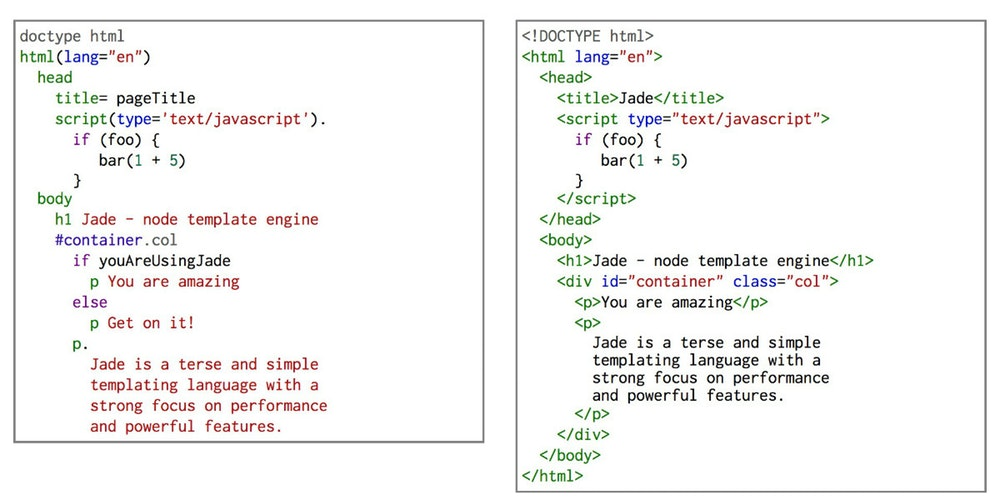
\includegraphics[width=1\linewidth]{bilder/pug}
	\caption[Pug im Vergleich zu HTML]{Pug im Vergleich zu HTML \cite{Janschltz2015}:\\Rechts abgebildet \texttt{Pug}, Links \texttt{HTLM}. Durch die Einrückung und dem Wegfall von schließenden Tags ist der Code deutlich übersichtlicher.}
	\label{fig:pug}
\end{figure}


 
Es werden anschließend für alle Models Views angelegt, damit Lehrende sich anmelden und einloggen, sowie neue Benutzer anlegen und editieren können. Ebenso für das Erstellen von Lehreinheiten mit den Unterrichtsmethoden Brainstorming und Quiz. Dabei werden bei Dateneingabe HTML-Formulare verwendet, welche anschließend via POST-Request an den Server geschickt werden. Controller validieren und werten diese folglich aus. Die Implementierung für das tatsächliche Ausführen der Unterrichtsmethoden wird in Abschnitt \ref{sec:implementclients} beschrieben. 

\subsection{UI Design}\label{sec:uidesign}
Aufbauend auf den Abschnitt \ref{sec:uientwurf} des Entwurf-Kapitels wird zur Designumsetzung das Frontend-CSS-Webframework \emph{Bootstrap} \cite{Twitter2019} genutzt. Dieses kann ebenfalls einfach über NPM dem Projekt hinzugefügt werden. Als Design-Theme bildet das frei erhältliche \emph{Bootstrap}-Theme \texttt{Neat} von \emph{freehtml5.co} die Grundlage (siehe Abbildung \ref{fig:screenshot_lehreinheiten}). Dieses wird hauptsächlich im Lehrerbereiches genutzt und in angepasster Version für den Student Client und den Presenter Client. Letzterer wird insbesondere für die Nutzung auf Großbildgeräten wie Fernsehern und Projektoren optimiert. Es wird sichergestellt, dass sich die Software angenehm auf stationären wie mobilen Endgeräten nutzen lässt. 

\begin{figure}[h!]
	\centering
	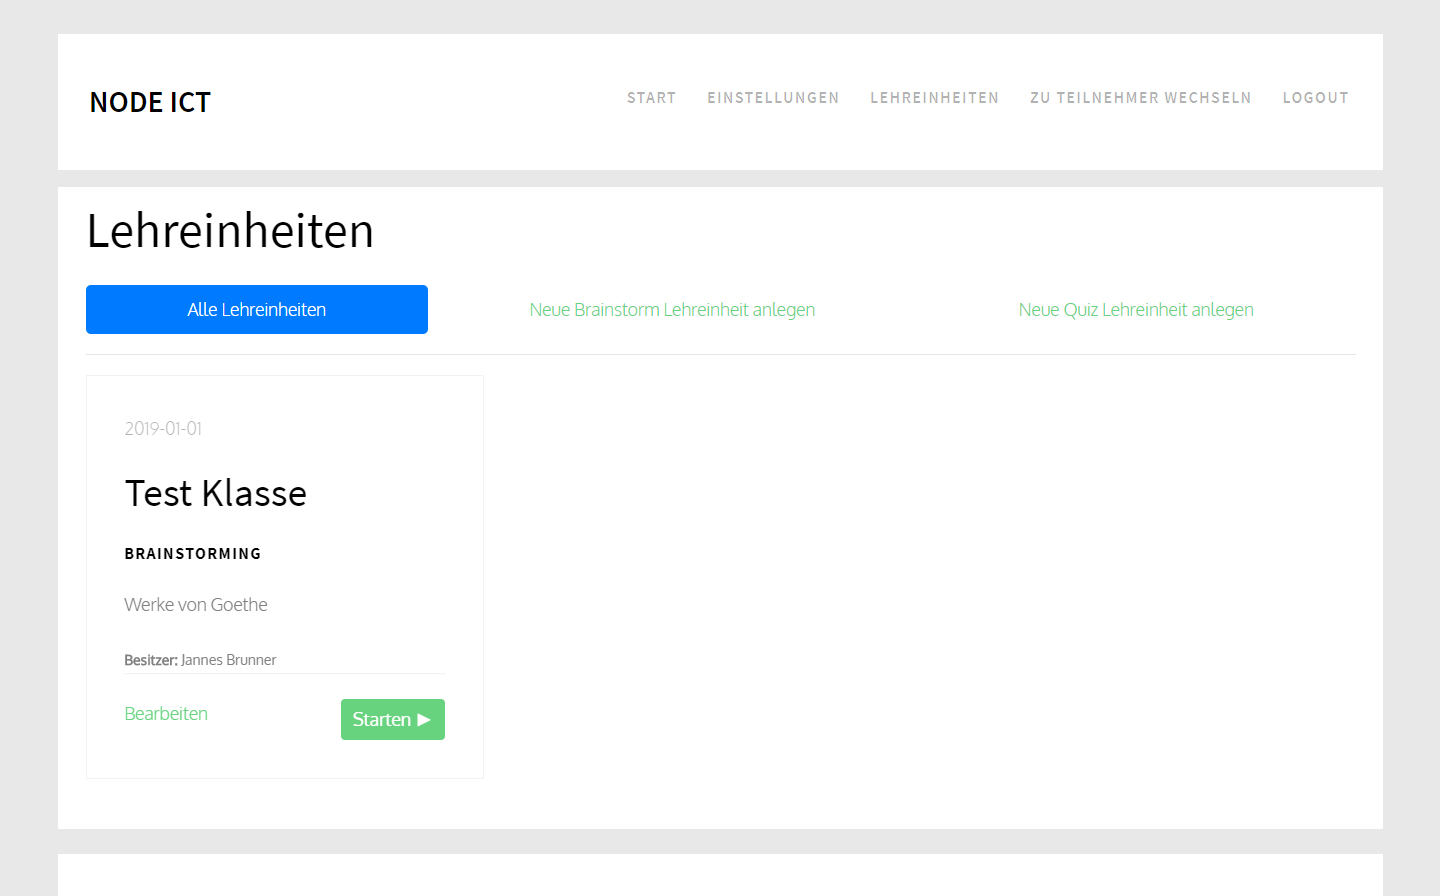
\includegraphics[width=0.9\linewidth]{bilder/screenshot_lehreinheiten}
	\caption[Screenshot UI Design Lehreinheitenbereich]{UI Design der Applikation beispielhaft illustriert durch ein Screenshot des Lehreinheiten Bereiches im Backend Zugang des Teacher Clients.}
	\label{fig:screenshot_lehreinheiten}
\end{figure}

\paragraph{Absicherung des Bereiches}
Bestimmte Bereiche der Applikation sollen nur registrierten und freigeschalteten Benutzenden zugänglich sein. Beim erstmaligen Initialisieren wird der Server mit einem Super-Administrator Account eingerichtet. Nur dieser soll neue Nutzer freischalten, andere Lehrende zu Administratoren ernennen und die Applikation auf Werkseinstellungen zurücksetzen können. Eine entsprechende Einrichtungsmaske soll beim ersten Serverstart automatisch erscheinen. Um dies technisch zu realisieren, wird das aus dem Kapitel \ref{sec:konzept} genannte \texttt{express-session} NPM-Modul genutzt, welches bereits vollständig mit der von \emph{Sequelize} verwalteten \emph{SQLite} Datenbank kompatibel ist. Nach der Einrichtung im Hauptmodul wird eine eigene Middleware-Funktion geschrieben, welche bei allen abgesicherten Routen als erstes aufgerufen wird und überprüft, ob die vom Client übertragene Session noch gültig ist.
\begin{lstlisting}[caption=Code der Authentifizierungs Middleware]
module.exports = (req, res, next) => {
	if(!req.session.isLoggedIn) return res.redirect('/teacher/login');
	next();
}
\end{lstlisting}
Falls dies nicht der Fall ist, wird auf die Login Seite verwiesen. 
Das Verwalten der Sessions und das Generieren von Cookies für die Client-Seite wird automatisch von dem Modul übernommen.
 \subsection{Umsetzung des Client Softwareanteile}\label{sec:implementclients}
 %Hier auch setup, browserify! 
 % vuejs, etc pp
Nachdem die Funktionen "`Erste Initialisierung der Software"', "`Login/Logout"' inkl. Benutzerverwaltung sowie das Anlegen und Verwalten von Lehreinheiten des Typs Brainstorming und Quiz implementiert sind, sollen die Lehreinheiten auch aktiv ausgeführt werden können. Dies bildet die Kernfunktion der Software und verlangt mehr Interaktion auf der Client Seite.\\ \\ 
\emph{Browserify} wird einfach über NPM dem Projekt hinzugefügt und ist anschließend einsatzbereit. Alle im Abschnitt \ref{sec:clientjs} des Kapitels Konzept erwähnten JS-Lösungen sind als NPM Modul verfügbar und werden ebenfalls dem Projekt hinzugefügt. Pro Client (Teacher Client, Student Client, Presenter Client) wird ein Development-Modul angelegt (\texttt{dev.js}). In diesem können alle benötigten JS-Bibliotheken normal importiert und genutzt werden. 
Via \emph{Browserify} wird anschließend pro Client ein Production-Modul generiert (index.js), welches alle notwendigen Importe bündelt. Um diesen Prozess zu automatisieren, wird ein Skript erstellt, welches vom NPM ausgeführt werden kann. Nur das Production-Modul muss via \texttt{script}-tag in das jeweilige \emph{Pug} Template pro Client eingebunden werden. Dies reduziert gleichzeitig die Anzahl notwendiger GET-Requests auf der Client-Seite. \\
Pro Client wird die UI mit dem JS-Framework \emph{Vue.js} kontrolliert und verwaltet. 
Auf dem HTML Layout wird ein \texttt{div}-Element als Ankerpunkt definiert und alle unterliegenden Elemente stehen fortan zur dynamischen Anpassung bereit. Mittels Datenbindung (Data-Binding) hält \emph{Vue.js} die angezeigten Informationen auf dem UI aktuell. \emph{Vue.js} ist dabei pro Client als einfaches JS Objekt auch von außen ansprechbar, was die Schnittstelle für andere Bibliotheken, insbesondere \emph{Socket.IO}, bildet. \emph{Socket.IO} auf der Client-Seite ist für den gesamten Datenverkehr zwischen Server und Client verantwortlich. Sowohl auf Server- wie auch Client-Seite können sog. "`Listener"' programmiert werden, die auf bestimmte Ereignisse (Events) von der, jeweils anderen Seite ausgelöst, lauschen. Im Ereignisfall wird eine anonyme Funktion aufgerufen, welche sich um die eintreffenden Daten kümmert. Die ausgetauschten Daten müssen hierbei nicht zwangsläufig zuvor in das  JSON-Format umgewandelt werden, wie dies sonst bei REST-Apis üblich ist. \\ \\ Auf der Server-Seite kümmert sich das Modul \texttt{ioSocketHandler.js} um alle eingehend Web-Socket Verbindungen und ordnet diesen zunächst einem Namensraum (Name\-space) zu. Ein Student Client wird dabei immer dem Namensraum für Student Clients zugeordnet und steht als Socket Objekt zur Verfügung, übliche Clients diesem Schema folgend.  Nach erfolgreicher Verbindung wird dem Student Client eine Liste verfügbarer Lehreinheiten geschickt und diesem auf der Client Seite dargestellt. Pro Lehreinheit (Typ Brainstorming oder Quiz) gibt es einen "`Session Handler"', der als JavaScript Klasse implementiert ist. Startet eine Lehrkraft eine Lehreinheit wird abhängig vom Typ eine neuen Klasseninstanz angelegt und eine Referenz in einem Speicher gehalten. Tritt nun ein Schüler der Lehreinheit bei, übergibt das übergeordnete "``Socket Handler"'-Modul das Socket-Objekt der Klasseninstanz der Lehreinheit. Die gesamte Logik und Kommunikation der auszuführenden Lehreinheit wird von der jeweiligen Klasse übernommen. Beendet eine Lehrkraft die Session, wird diese aus dem Speicher entfernt und steht nicht mehr zum Beitreten zur Verfügung. Pro gestartete Session kann über einen speziellen Link der passende Presenter Client aufgerufen werden. Dieser wird ebenfalls über das \texttt{ioSocketHandler.js} Modul der jeweiligen Klasseninstanz zugeordnet. Im Listing 8 wird ein Codeauszug gezeigt, welcher den Datenaustausch zwischen Server und Client zeigt.
\begin{lstlisting}[caption=Server Socket Event-Emitierung]
/// TEACHER :::::::
updateSessionT() {
	this.socketT.emit("updateSession", this.session);
}
\end{lstlisting}

Der Server schickt das Event \texttt{updateSession} an den Teacher Client.
Als Inhalt der Nachricht wird das Session Objekt (\texttt{this.session}) übermittelt.
\begin{lstlisting}[caption=Client Socket Event-Listener]
// Sever tells client to update the session object
socket.on("updateSession", function (newSession) {
	console.log("getting fresh session from server...", newSession)
	if (newSession && newSession.id == vue.session.id) {
		vue.session = newSession;
	}});
\end{lstlisting}

Der Teacher Client lauscht auf das Event \texttt{updateSession}. Trifft dieses ein,
wird eine anonyme Funktion aufgerufen, welche sich dem Inhalt der Nachricht annimmt.
Diese überprüft in diesem Fall zunächst, ob sich die ID des zu aktualisierenden Session Objekts
mit dem ursprünglichen deckt. Anschließend wird das alte Session Objekt auf das neue referenziert.  
 
\subsection{Herausforderungen der Implementierung}\label{sec:probsserver}
%ioSessionHandler Socket Handling
%Word Cloud passende finden und praktikabel 
%Wifi Hotspot node module 
%Allgemeiner Umfang von VueJS und sein Einsatz
Während der Implementierung stellte sich anfangs das Verbindungsmanagement der verbundenen Clients über \emph{Socket.IO} als instabil heraus, da Sockets sich bei Verbindungsabbruch zwar selbständig erneut verbinden, jedoch immer unter einer neuen Session ID. Dies führte zunächst zu unerwartetem Verhalten während einer Lehreinheiten Ausführung. Dem konnte aber durch zusätzliche Authentifizierungsdaten entgegengewirkt werden. Bei mobilen Geräten wie Smartphones erwies sich der Verbindungsabbruch zusätzlich als geräteabhängig. Manchen Geräten unterbrechen die Verbindung z.B. beim Ausschalten des Bildschirms sofort, während andere diese im Hintergrund weiterhin aufrecht erhalten. \\ Außerdem war es schwierig ein gut funktionales "`Word-Cloud / Wörterwolke"'-Modul zu finden, welches sich ohne nennenswerte Probleme mit \emph{Vue.js} im Einklang nutzen lassen konnte. Generell wird \emph{Vue.js} in diesem Projekt recht rudimentär eingesetzt, was seine Funktionsweise zwar nicht einschränkt, jedoch das volle Potential dieser Web-Frontend-Engine nicht gänzlich nutzt. \\ \\ Das NPM-Modul \texttt{node-hotspot} wurde zwar gemäß der Instruktionen der Entwickler implementiert, allerdings konnte auf mehreren \emph{Microsoft Windows} Testsystemen nicht selbstständig ein WLAN-Hotspot aktiviert werden. Leider war \texttt{node-hotspot} zum Entwicklungszeitpunkt (Stand Juli 2019) das einzige verfügbare NPM-Modul, welches die Generierung eines WLAN-Hotspots bezweckte. 
 
 
 